% =============================================================================================
% SECTION 2 -- METHODS.
%
% Condensed 2026-10-05 (research-paper pass). The detailed curation rules, the reference-choice
% ladder, the quality-control gates, the pairing rules, the boundary-scattering bound, the
% structure-only search procedure, the populations table and the training-data figure moved to the
% Supplementary material, section "Extended Methods" (sec:extmethods there). Each is summarised
% here in one or two sentences with a pointer.
%
% Every number below is a key of data/exports/kappa_v2/paper_numbers.json, or arithmetic on such
% keys (284/50 = 5.7; 1 - c = 0.58; 10^0.270 = 1.86; interval coverage counts = coverage x 39), or a
% threshold defined in code.
%   9495 / 960 / 735 / 152        corpus.rows_all / compounds_all / half_heuslers /
%                                 source_dois_behind_measured
%   681 / 463 / 284 / 230         training_data.n_labels / n_compounds / n_half_heusler /
%                                 n_half_heusler_vec18
%   544 at 300 K, 119 at 500 K    training_data.labels_by_T
%   45 descriptors; 81 missing    shap_ranking.n_descriptors; shap_ranking.top[bond_min].n_missing
%   R2 / RMSE / MAE / median err  model_comparison.{catboost,lightgbm,gpr,krr}.*
%   2.18                          cap_test.max_uncapped_factor
%   0.41-0.56 / 0.50-0.80 etc.    calibration.stability (leave-one-cluster / -family / bootstrap)
%   Gemini models, counts, dates  extraction database (FIX_DECISIONS.md, journal compliance)
%   VEC counting rule             make_paper_predictions.ve / vec (pymatgen group; lanthanides and
%                                 actinides carry group 3)
%   100 K temperature bin         run_target_blind_test.py (Tbin = round(T/100)*100)
%   bands 1.62/2.56/2.85 etc.     conformal_indomain (seed medians, coverage counts)
% =============================================================================================

\section{Methods}
\label{sec:method}

We aim to predict the \emph{measured} lattice thermal conductivity, $\kappa_L$, of half Heuslers. A
machine-learning model predicts the first-principles (Boltzmann-transport-equation, BTE)
conductivity, $\kappa_L^{\mathrm{BTE}}$, from the crystal structure (Section~\ref{sec:model}), and a
transfer function maps any first-principles value onto the experimental scale
(Section~\ref{sec:transfer}). Where a published calculation exists, the transfer function is applied
to it directly and the model is not used. Figure~\ref{fig:method} shows the procedure: measurements
and calculations stay in separate tracks from the corpus onward and meet only at the transfer
function. Rules stated here only in outline are given in full in the Extended Methods
(Section~S12 of the Supplementary material).

\paragraph{Notation and conventions.} We write $\kappa_L^{\mathrm{BTE}}$ for a calculated
conductivity and $\kappa_L^{\mathrm{exp}}$ for a value on the experimental scale, whether a
measurement or a calculation mapped onto that scale. A half Heusler is written XYZ, with X the most
electropositive element (a rare earth or an early transition metal), Y the late transition metal and
Z the main-group element. A \emph{bonding family} is the pair of elements on the Y and Z sites,
labelled by those two elements, as in the \ce{Sb}--\ce{Pt} family; neither the order of the two
symbols nor the order of the elements in a formula carries meaning. Each prediction for an
unmeasured compound carries one of three \emph{statuses} (Section~\ref{sec:screening}):
\emph{issued}, a prediction this paper makes; \emph{flagged}, a calibrated value declined because it
fails a named check; and \emph{conditional}, an estimate on the shared constant in a family with no
usable measured member. The word \emph{tier} is reserved for the method tiers 0--3 of
Section~\ref{sec:tiering}. The \emph{deployed} constants are those used for the issued predictions.

\begin{figure*}[tbp]
  \centering
  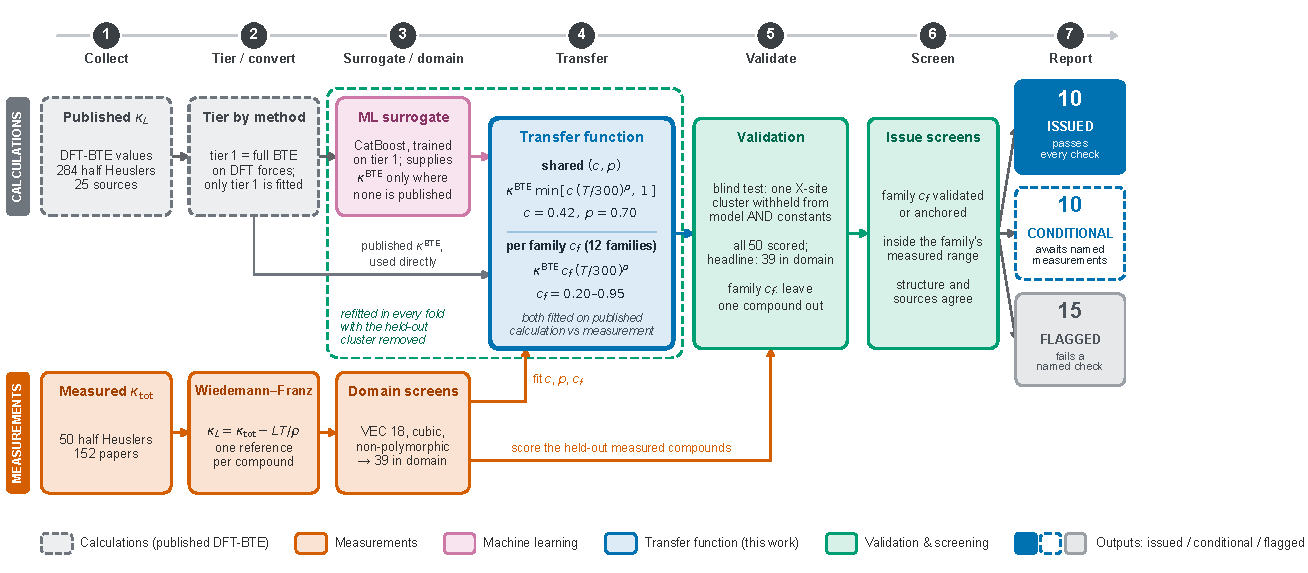
\includegraphics[width=\linewidth]{figures/fig08_method.pdf}
  \caption{\textbf{The method, end to end, in seven numbered steps.} Calculations (upper lane, grey,
  dashed) and measurements (lower lane, orange) are tiered, converted and screened separately, and
  meet only at the transfer function (blue). A published full Boltzmann-transport calculation
  (tier~1) is corrected directly; the machine-learning surrogate (pink), trained on tier~1 only,
  supplies a calculation only where none is published. The measurements fit the shared constants
  ($c$, $p$) and the per-family constants $c_f$, and separately score the held-out compounds. The
  green dashed region marks what each fold of the blind test refits with one X-site chemistry
  cluster removed. Predictions that pass the issue screens are issued; a prediction that fails a
  named check is flagged; estimates on the shared constant, in families with no usable measured
  member, are conditional.}
  \label{fig:method}
\end{figure*}

\subsection{Corpus construction}
\label{sec:dataset}

A correction from calculation to experiment can be fitted only on compounds that have both, so the
corpus records calculations and measurements separately. It holds \num{9495} temperature-resolved
values for \num{960} distinct Heusler compounds, \num{735} of them half Heuslers, and every value
records its source and how it was obtained.

Experimental values come from the Starrydata curated transport database~\cite{katsura2025starrydata},
read at its published snapshot of 1 July 2025~\cite{mato2025starrydata}, and from direct extraction
from primary publications. Starrydata aggregates curves digitised from primary publications; the
measured half-Heusler values trace to \num{152} distinct publications. For direct extraction,
multimodal large language models read the full text, tables and figures: Google Gemini
\texttt{gemini-2.5-flash} (\num{483} extractions, 4--13 July 2026) and \texttt{gemini-2.5-pro}
(\num{695} extractions, 13 July -- 18 September 2026). A retrieved record with no body text is never
passed to the model, and every extracted value must pass the physical and provenance gates below,
so no value enters the corpus on the model's authority alone. First-principles values come from
AFLOW~\cite{curtarolo2012aflow} (its AAPL transport module~\cite{plata2017an} and its AGL
Debye--Gr\"{u}neisen estimates~\cite{toher2014highthroug}, kept apart by the tiering below), the
Materials Project~\cite{jain2013commentary}, JARVIS~\cite{choudhary2020the},
OQMD~\cite{kirklin2015the} and published phonon-transport studies. Crystal structures come from the
same repositories, the Crystallography Open Database~\cite{graulis2009crystallog} and
OPTIMADE-federated sources~\cite{andersen2021optimade}.

Experiments measure the total thermal conductivity, so most measured rows separate the lattice part
by Wiedemann--Franz subtraction,
%
\begin{equation}
  \kappa_L = \kappa_\mathrm{tot} - \frac{L T}{\rho},
  \label{eq:wf}
\end{equation}
%
with the Lorenz number $L$ from the single-parabolic-band parameterisation of Kim and
Snyder~\cite{kim2015characteri}, $T$ the temperature and $\rho$ the electrical resistivity; every
row records which route produced it. Because Eq.~\eqref{eq:wf} is a difference of two measured
quantities, $\rho$ must lie in the range available to a dense intermetallic; a row outside it
reports total conductivity under a lattice label and is removed. Four further rules decide what
counts as a measurement: a value one paper quotes from another is not one; a sample digitised twice
enters once; a data deposit that republishes curves is never counted as a laboratory; and a
composition must be a Heusler. A separate gate collapses a preprint, a deposit and the article they
duplicate onto the version of record, so that one calculation is never counted as two groups. The
rules are given in full in the Extended Methods.

Figure~\ref{fig:corpus} summarises the corpus. Of the \num{735} half Heuslers with any
thermal-conductivity record, \num{284} have a full transport calculation and \num{50} have been
measured, and the evidence behind the measured set is uneven: many compounds rest on a single
publication, a few on ten or more.

\begin{figure*}[tbp]
  \centering
  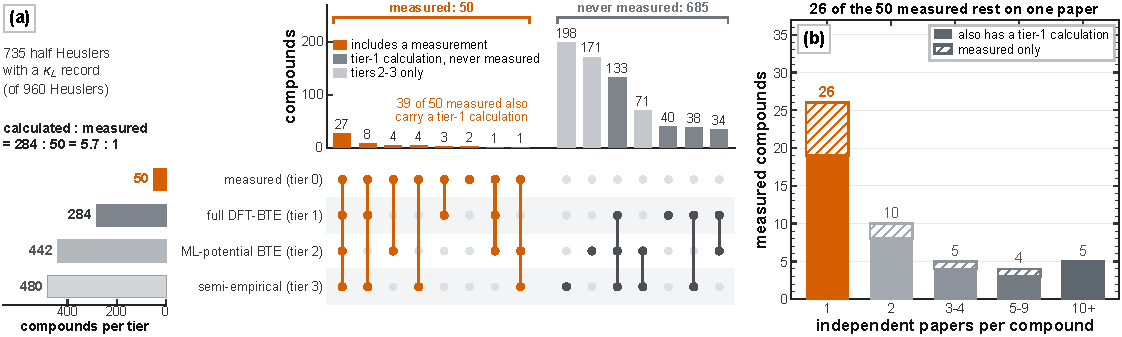
\includegraphics[width=\linewidth]{figures/fig01_corpus.pdf}
  \caption{\textbf{The half-Heusler $\kappa_L$ corpus.} (a)~The \num{735} half Heuslers with a
  thermal-conductivity record (of \num{960} Heusler compounds) by evidence type: rows are method tiers
  (measured; full DFT-BTE; ML-potential BTE; semi-empirical), columns the tier combinations
  compounds carry; column heights give compound counts and left bars tier sizes. \num{284} compounds
  carry a full calculation and \num{50} a measurement (\num{5.7}:1); \num{39} of the \num{50} also
  carry a tier-1 calculation (not the same set as the \num{39} in-domain compounds of the blind
  test). (b)~Independent publications per measured compound, a preprint and its article counted
  once; hatched, no tier-1 calculation. \num{26} of the \num{50} rest on a single publication.}
  \label{fig:corpus}
\end{figure*}

\subsection{The measured values and the choice of reference}
\label{sec:measured}

A transfer function is only as well defined as the experimental scale it maps onto. Every reference
is a stoichiometric parent compound (each coefficient within \num{0.02} of an integer), so the
doped and alloyed specimens that dominate the half-Heusler literature are excluded and the
correction measures the offset between a calculation and a measurement of the same compound. That
offset still has two sources, which we do not separate: error in the calculation itself (a
three-phonon calculation omits higher-order scattering, and the exchange-correlation functional is
approximate) and the specimen, whose point defects, grain boundaries and incomplete density are
absent from the calculation of a perfect crystal.

We never blend the curves of several laboratories, since a blend is a curve nobody measured. A fixed
ladder, reading only the specimen and the temperature coverage of each measurement and never a
calculation, chooses one reference laboratory per compound: the central laboratory when four or more
report it, otherwise the densest specimen, otherwise the widest temperature range. A
\emph{family-paper rung} makes one primary publication that measured two or more members of a family
the reference for those members, so that a family constant describes one kind of specimen. A
laboratory contradicting a consensus, a data deposit, a nanostructured specimen and a source with
fewer than four temperatures rank last but are never deleted, and a curve-shape test rejects curves
with a visibly mis-subtracted electronic term (full rules in the Extended Methods). Within the chosen
publication, the value in each \SI{100}{\kelvin} temperature bin is the median of its rows. In the
blind test, and for the compound held out in the family test, the reference is chosen without the
family-paper rung, so that it never depends on which siblings have been measured. The sources record
little about each specimen, and independent laboratories measuring the same compound disagree by a
median factor of \num{1.33}; the correction is therefore not a microstructural model but the expected
value over published practice, and every score depends on the choice of reference as well as on the
method.

\subsection{Method tiers and quality control}
\label{sec:tiering}

Every row carries a \emph{method tier}. Tier~0 is a laboratory measurement (\num{50} half Heuslers
from \num{152} publications). Tier~1 is a full solution of the phonon Boltzmann transport equation
from first-principles third-order force constants (\num{284} half Heuslers). Tier~2 is an
approximate or reduced transport route, including a transport calculation whose force constants come
from a machine-learned interatomic potential. Tier~3 is a semi-empirical or quasi-harmonic estimate:
Slack~\cite{slack1979the}, Debye--Callaway~\cite{callaway1959model} or AGL. Only tier~1 enters the
calibration and, for half Heuslers, the training of the regression model. The tier is assigned from
the method string, never from a repository's label, and tier~1 requires a positive match for a
transport solution with no disclaimer attached.

Five quality-control conditions are applied when the corpus is generated: a cubic $C1_b$ record
(space group 216) from a source that is not a prototype-substitution database; a polymorph flag for a
compound also recorded in a non-cubic space group; separation of half from full Heuslers by the site
ratio; a \SI{200}{\kelvin} temperature floor, below which a boundary-free calculation and a
boundary-limited measurement are not the same quantity; and a transport-calculation method string
for tier~1. They are stated with their reasons in the Extended Methods.

\subsection{Domain of applicability}
\label{sec:domain}

A transfer function for \emph{lattice} thermal conductivity is meaningful only where lattice
conduction dominates. The domain is half Heuslers with 18 valence electrons, a cubic $C1_b$
structure, and no other polymorph on record. Transition-metal half Heuslers are semiconducting at a
valence-electron count (VEC) of 18~\cite{graf2011simple}; away from it a large electronic term must
be removed from every measurement. VEC sums, over the three elements of the 1:1:1 formula, the group
number for groups 1--12 and the group number minus 10 for groups 13--18, with lanthanides and
actinides counted as group~3. We restrict to $\mathrm{VEC}=18$ because that is where the corpus has
support. The structural conditions follow because the calculation being calibrated is for the cubic
phase.

Two further screens apply to prediction candidates only. A candidate containing \ce{Ce}, \ce{Sm},
\ce{Eu} or \ce{Yb}, whose valence is not fixed~\cite{lawrence1981valence}, is flagged rather than
issued (the validation compound \ce{YbNiSb} is still scored), and a candidate containing a
radioactive element is excluded, since the corpus holds no training example of one.

All \num{50} measured half Heuslers are scored in the blind test; \num{44} have $\mathrm{VEC}=18$ and
\num{39} also pass the structural conditions, forming the in-domain set. The domain is defined by the
screens every candidate must pass, independently of the validation result, and the headline and its
null comparison are reported with and without the screens (Section~\ref{sec:blind}). Other
sub-populations are defined where they first appear and tabulated in the Extended Methods; figures
over different populations are not directly comparable.

\subsection{Training data, descriptors and the machine-learning model}
\label{sec:trainingdata}
\label{sec:model}

The model learns calculations, never measurements. Its label is the phonon Boltzmann-transport
conductivity of a cubic crystal,
%
\begin{equation}
  \kappa_L^{\mathrm{BTE}} \;=\; \frac{1}{3N_{\mathbf{q}}V}\sum_{\mathbf{q},s}
    C_{\mathbf{q}s}\, v_{\mathbf{q}s}^{2}\, \tau_{\mathbf{q}s},
  \label{eq:bte}
\end{equation}
%
a sum over the $N_{\mathbf{q}}$ sampled wavevectors $\mathbf{q}$ and branches $s$ of the mode heat
capacity $C_{\mathbf{q}s}$, squared group velocity $v_{\mathbf{q}s}^{2}$ and lifetime
$\tau_{\mathbf{q}s}$, divided by the cell volume $V$. The training pool holds \num{681} labels on
\num{463} compounds. Of these, \num{284} are half Heuslers (\num{230} with $\mathrm{VEC}=18$), each
labelled by a full first-principles calculation; tier-2 and tier-3 half-Heusler values are excluded.
Full Heuslers share the descriptors and enter the pool, those without a transport calculation
through a semi-empirical estimate at reduced weight; held-out scoring always uses half Heuslers
alone. Of the labels, \num{544} are at \SI{300}{\kelvin} and \num{119} at \SI{500}{\kelvin}, so the
training data constrain the temperature dependence only weakly. The labels are strongly
right-skewed, so the model is fitted on $\log_{10}\kappa_L^{\mathrm{BTE}}$; their distribution is
shown in the Extended Methods.

We train gradient-boosted decision trees (CatBoost~\cite{prokhorenkova2017catboost}). Each prediction
is the median over five random seeds. Some diagnostics are run at one seed, always seed~0, the
\emph{reference seed}, and are labelled as such; headline figures are medians over the five seeds.

\paragraph{Descriptors.} Each row is described by \num{45} descriptors of the composition, the cubic
cell and the temperature, in six groups: (i)~site properties (mass, radius and electronegativity of
X, Y and Z); (ii)~cross-site means, contrasts, spreads and ratios, including the X--Z
electronegativity difference; (iii)~Klemens-type disorder, zero throughout this stoichiometric pool
and kept only so the set is defined for substituted compositions; (iv)~cell geometry (volume per atom,
density, atoms per conventional cell, full-Heusler and quaternary flags); (v)~bond lengths from the
atomic coordinates, missing for \num{81} rows and handled natively by the model; and
(vi)~temperature, as $T$, $1000/T$ and $\log_{10}T$. The lattice parameter itself is never a
descriptor, because sources mix the primitive and conventional cells.

\subsection{Model selection}
\label{sec:modelselection}

We compared four regressors on identical rows, descriptors and weights: CatBoost, LightGBM, a
Gaussian process and kernel ridge regression, each scored out of fold on the full pool with
five-fold cross-validation grouped by element system. CatBoost has the highest $R^2$ and the lowest
RMSE and MAE (Table~\ref{tab:models}); LightGBM has the lowest median error per compound, by
\num{0.1} percentage points (pp), too small to separate the two, and we retain CatBoost. Only kernel
ridge falls clearly behind, so the results do not hinge on the choice. The comparison measures fit to
calculated labels, on element-system folds rather than the X-site clusters of the validation, and
over the whole pool, so its figures are not comparable with the half-Heusler accuracy of
Section~\ref{sec:mlrepro}. Parity plots for all four are in Section~S7 of the Supplementary
material.

\begin{table}[tbp]
  \centering
  \caption{Model selection: four regressors trained on identical rows (\num{681} rows, \num{463}
  compounds) and scored out of fold on identical element-system folds. RMSE, MAE and $R^2$ are per
  row on $\log_{10}\kappa_L$; the median error is per compound
  (Section~\ref{sec:metrics}). The retained model is in bold.}
  \label{tab:models}
  \small
  \begin{tabular}{lcccc}
    \toprule
    Regressor & RMSE & MAE & $R^2$ & median error \\
    \midrule
    \textbf{CatBoost}  & \textbf{\num{0.270}} & \textbf{\num{0.182}} & \textbf{\num{0.701}} & \SI{26.1}{\percent} \\
    LightGBM           & \num{0.273} & \num{0.186} & \num{0.695} & \SI{26.0}{\percent} \\
    Gaussian process   & \num{0.281} & \num{0.190} & \num{0.676} & \SI{26.4}{\percent} \\
    Kernel ridge       & \num{0.343} & \num{0.236} & \num{0.516} & \SI{32.3}{\percent} \\
    \bottomrule
  \end{tabular}
\end{table}

\subsection{The transfer function}
\label{sec:transfer}

A first-principles calculation describes a perfect, infinite crystal; a laboratory specimen is a
polycrystal with grain boundaries, point defects and finite density, each of which scatters phonons
the calculation lets propagate freely. For the \ce{XNiSn} half Heuslers this has been analysed directly
against measurement~\cite{schrade2017the}. The measured conductivity is therefore lower, and the
specimen contribution would be expected to grow as temperature falls and the intrinsic mean free
path grows.

\paragraph{The shared form.} We describe the offset empirically with two parameters:
%
\begin{equation}
  \kappa_L^{\mathrm{exp}}(T) \;=\; \kappa_L^{\mathrm{BTE}}(T)\;
    \min\!\left[c\left(\frac{T}{300}\right)^{p},\,1\right].
  \label{eq:transfer}
\end{equation}
%
Here $c$ sets the room-temperature reduction and $p$ its temperature dependence. The cap at one is a
modelling choice for the shared form, which keeps a calibrated value from exceeding its calculation;
it is not a physical requirement, since part of the offset is error in the calculation, which can
have either sign. The constants are fitted on published tier-1 calculations, each paired with the
reference measurement of the same compound, with no regression model involved. Such pairs exist for
\num{34} in-domain compounds (\num{429} pairs). We fit per compound,
%
\begin{equation}
  (c, p) \;=\; \operatorname*{arg\,min}_{c,\,p}\;
    \operatorname*{median}_{i \in \mathcal{C}}\;
    \operatorname*{median}_{j}
    \left|\log_{10}\frac{\hat{\kappa}(T_{ij};c,p)}{\kappa(T_{ij})}\right|,
  \label{eq:fit}
\end{equation}
%
where $\mathcal{C}$ is the set of compounds with pairs that remain after the scored compound's
\emph{held-out unit} is removed, $\hat{\kappa}$ is the corrected calculation and $\kappa$ the
reference measurement at the matched temperatures $T_{ij}$. The held-out unit is the X-site
chemistry cluster in the blind test, the bonding family in the unseen-family test, and the compound
itself in the family comparison (Section~\ref{sec:nulls}), so no scored compound informs the
constant applied to it. The error is taken in logarithm because it is multiplicative, and medians
stop a single digitisation artefact from steering the fit. On all \num{34} compounds the fit gives
the deployed $c=\num{0.42}$ and $p=\num{0.70}$; $c\,(T/300)^{p}$ then reaches one at
\SI{1036}{\kelvin}.

The magnitude is well determined and the exponent is not. Removing any one of the \num{16} chemistry
clusters among the \num{34} compounds moves $c$ within \numrange{0.41}{0.56} and $p$ within
\numrange{0.50}{0.80}; removing any one of the \num{12} bonding families moves $c$ within
\numrange{0.40}{0.54} and $p$ within \numrange{0.60}{0.80}. Over \num{200} bootstrap resamples of the
compounds, the 10th--90th percentile range is \numrange{0.35}{0.55} for $c$ but \numrange{0.45}{1.15}
for $p$. We therefore do not claim to predict the temperature dependence of an individual compound.

\paragraph{The family form.} Every bonding family with at least one member that has both a published
calculation and a usable reference measurement carries its own constant:
%
\begin{equation}
  \kappa_L^{\mathrm{exp}}(T) \;=\; \kappa_L^{\mathrm{BTE}}(T)\;
    c_f\left(\frac{T}{300}\right)^{p}, \qquad p = \num{0.70}.
  \label{eq:family}
\end{equation}
%
Twelve families qualify. Only the magnitude is refitted, by Eq.~\eqref{eq:fit} restricted to
$c_f<1$ on the family's measured members, because most families are measured over too narrow a
range to identify their own exponent. A family with two or more measured members (nine families) is
tested held out, each member predicted from the others with its own measurement withheld, and
\emph{passes}, or is \emph{validated}, only if the median error over its folds is under
\SI{25}{\percent}. A family with one member is \emph{anchored}: its figure is an in-sample fit,
never a validation. The family form carries no cap and can exceed its calculation at high
temperature, by up to \num{2.18} times, which is where the measurements of those families lie; every
issued prediction carries a factor below one.

A compound receives its family's constant wherever its family has a measured member, and the shared
constant otherwise. The leave-one-chemistry-out blind test is the exception: it is scored with the
shared constant, because a chemistry holdout leaves a compound's family-mates in training and would
not test a family constant at all.

\paragraph{Pairing a calculation with a measurement.} A calculation reported at several temperatures
is interpolated in log--log space; one reported at a single temperature is carried as
$\kappa_L^{\mathrm{BTE}} \propto 1/T$, the high-temperature limit of three-phonon Umklapp
scattering, by no more than a factor of \num{2.5} in temperature and never below
\SI{200}{\kelvin}. Independent calculations are combined by their median, and a temperature at which
they disagree by more than a factor of two is \emph{contested} and not used, for measured compounds
and candidates alike; this is why \ce{TiNiPb} is quoted at \SI{500}{\kelvin}. The full rules are in
the Extended Methods.

\paragraph{What the constants mean.} Empirical temperature dependences have been fitted to measured
half-Heusler curves before~\cite{geng2014lattice,petersen2015critical}; here we fit instead the
\emph{ratio} of measurement to calculation, and this work adds the corpus, the class-wide magnitude
and the held-out validation, not the functional form. With $\kappa_L^{\mathrm{BTE}} \propto T^{-1}$,
$p=\num{0.70}$ implies a corrected $\kappa_L \propto T^{-0.30}$. The correction is empirical, not a
boundary-scattering term: a single-boundary-length model, grey or spectral~\cite{callaway1959model},
caps the logarithmic slope of the suppression at $1-c$ (\num{0.58} at $c=\num{0.42}$), and the fitted
$p$ exceeds that cap, although its bootstrap range straddles it (derivation in the Extended Methods).
We attach no mechanism to the parameters.

\subsection{Predictions from crystal structure alone}
\label{sec:structureonly}

For a compound nobody has calculated, the model supplies $\kappa_L^{\mathrm{BTE}}$ and the transfer
function maps it onto the experimental scale. We searched DxMag~\cite{xiao2026accurate}, AFLOW, OQMD,
JARVIS and the Materials Project for cubic $C1_b$ cells inside the domain, took the lattice parameter
of the lowest-energy site ordering on record, and predicted a candidate only if its family, its X
element and every element are represented among the training half Heuslers. A prediction is graded
\emph{strong} when the model reproduces the family's own published calculations to within
\SI{25}{\percent} held out and the five seeds agree within a factor of \num{1.3}, \emph{moderate}
within \SI{50}{\percent} and \num{1.5}, and \emph{weak} otherwise. Literature status was checked in
OpenAlex~\cite{priem2022openalex}, Crossref and arXiv with a positive control; a value reported only
in a table or supplement is invisible to this search, which limits every novelty statement here. The
two steps, structure to calculation and calculation to experiment, carry errors that we report side
by side and never combine. The full procedure and two model-free cross-checks are in the Extended
Methods.

\subsection{Validation, null baselines and prediction intervals}
\label{sec:nulls}
\label{sec:intervals}

The evaluation rules for the results reported here were fixed in writing before this evaluation was
run: the definition of the shared constant and its held-out use, the single-reference rule, the
construction of the intervals at the quoted temperature, and the list of figures to be reported
whatever they showed. These documents are kept, time-stamped, in the code repository.

Every figure for the model route is obtained with the target compound's \emph{entire chemistry}
withheld: compounds are clustered by their X element and a whole cluster is removed at once
(\emph{leave-one-chemistry-out}), from the model and from the shared constant alike. Family-mates
with a different X element remain in training, so the test measures accuracy for a new X-site
substitution within a known family. There are \num{27} clusters among the \num{230} calculated
$\mathrm{VEC}=18$ half Heuslers, \num{16} among the \num{34} compounds of the published route,
\num{18} among the \num{39} in-domain compounds and \num{21} among all \num{50} measured ones. Every
threshold or model choice is made on one half of the clusters and evaluated on the other, and every
headline figure is the median over five model seeds, quoted with its range. Two \emph{null
baselines} use no compound-specific information: a constant equal to the median measured
conductivity of the training compounds, and a power law $A(T/300)^{q}$ fitted to them, both with the
same chemistry held out and the same references; the paired comparison is also made with each
cluster counted once. Family constants are tested leave-one-compound-out against the shared constant
refitted without the same compound, and the shared constant on families never measured is tested
leave-one-family-out on the \num{34} compounds of the published route.

Prediction intervals are split conformal intervals~\cite{lei2018distributi}, built from out-of-fold
residuals in logarithmic space. Each in-domain compound contributes one residual, under the
calibration it would actually receive (its family constant fitted without it, or else the shared
constant refitted without its cluster), in the temperature bin nearest the quoted temperature. For a
nominal level $\alpha$ over $m$ held-out compounds,
%
\begin{equation}
  \delta_\alpha \;=\; \Bigl\{\, \bigl|\log_{10} \rho_i \bigr| \,\Bigr\}_{(k)},
  \qquad k = \bigl\lceil (m+1)\,\alpha \bigr\rceil,
  \label{eq:conformal}
\end{equation}
%
where $\rho_i$ is the ratio of prediction to reference for compound $i$ in that bin and the band is a
factor of $10^{\delta_\alpha}$ either way. Exchangeability of the residuals is assumed, not shown,
and compounds sharing a cluster or a laboratory weaken it, so coverage is treated as a measured
frequency, evaluated leave-one-chemistry-out for each seed; the median band over seeds is deployed.
At \SI{300}{\kelvin} the bands are a factor of \num{1.62}, \num{2.56} and \num{2.85} at
\SI{50}{\percent}, \SI{80}{\percent} and \SI{90}{\percent} nominal, covering \num{20}, \num{31} and
\num{36} of the \num{39} in-domain compounds; at \SI{500}{\kelvin} they are \num{1.38}, \num{1.70}
and \num{1.89}, covering \num{20}, \num{32} and \num{36} (binomial uncertainty roughly
\SI{8}{pp}). Coverage is not validated for an anchored family or a family never measured.

\subsection{Metrics}
\label{sec:metrics}
\label{sec:definitions}

Model selection scores the fit to calculated labels \emph{per row}, on $y=\log_{10}\kappa_L$. Over
$N$ rows with labels $y_k$, out-of-fold predictions $\hat{y}_k$ and label mean $\bar{y}$,
%
\begin{gather}
  \mathrm{RMSE} = \sqrt{\frac{1}{N}\sum_{k=1}^{N}\bigl(\hat{y}_k-y_k\bigr)^2},
  \qquad
  \mathrm{MAE} = \frac{1}{N}\sum_{k=1}^{N}\bigl|\hat{y}_k-y_k\bigr|,
  \label{eq:rmse}\\
  R^2 = 1-\frac{\sum_k\bigl(\hat{y}_k-y_k\bigr)^2}{\sum_k\bigl(y_k-\bar{y}\bigr)^2};
  \label{eq:r2}
\end{gather}
%
an RMSE of \num{0.270} on the logarithm corresponds to a typical scatter by a factor of
$10^{0.270}\approx\num{1.86}$. Every other figure, including every comparison with measurement, is
reported \emph{per compound}. The error of a prediction $\hat{\kappa}$ at temperature $T$ against the
reference $\kappa$ is
%
\begin{equation}
  \mathrm{APE}(T) \;=\; \frac{\bigl|\hat{\kappa}(T) - \kappa(T)\bigr|}{\kappa(T)},
  \label{eq:ape}
\end{equation}
%
and for compound $i$ with matched temperatures $T_{ij}$,
%
\begin{equation}
  e_i \;=\; \operatorname*{median}_{j=1\ldots n_i} \mathrm{APE}(T_{ij}),
  \qquad
  r_i \;=\; \operatorname*{median}_{j} \frac{\hat{\kappa}(T_{ij})}{\kappa(T_{ij})}.
  \label{eq:err}
\end{equation}
%
We report the \emph{median error}, $\operatorname{median}_i e_i$; the fractions \emph{within a
factor of two} ($\tfrac{1}{2} \le r_i \le 2$), \emph{within \SI{30}{\percent}} ($e_i \le 0.30$) and
\emph{within \SI{25}{\percent}} ($e_i < 0.25$, the bar a family must pass); and the \emph{bias},
$\operatorname{median}_i r_i$. Aggregating per compound stops a compound measured at many
temperatures from outweighing one measured at few, and the calibration is fitted per compound for
the same reason. Differences between percentages are given in percentage points (pp).
